\documentclass{article}
\usepackage[utf8]{inputenc}
\usepackage[german]{babel}
\usepackage{amsmath,amsthm,amssymb,mathrsfs}
\usepackage{geometry}
\usepackage[shortlabels]{enumitem}
\usepackage{wrapfig}
\usepackage{xcolor}
\usepackage{chemformula}

% For images
\usepackage{graphicx}
\usepackage{subcaption}
\graphicspath{ {./} }

% For tables not moving around
\usepackage{float}
\restylefloat{table}


\newcommand{\N}{\mathbb{N}}
\newcommand{\Q}{\mathbb{Q}}
\newcommand{\Z}{\mathbb{Z}}
\newcommand{\A}{\mathbb{A}}
\newcommand{\R}{\mathbb{R}}
\newcommand{\C}{\mathbb{C}}

\renewcommand{\i}{\text{i}}

\newcommand{\mat}[1]{\left(\begin{matrix}#1\end{matrix}\right)}
\newcommand{\smat}[1]{\left(\begin{smallmatrix}#1\end{smallmatrix}\right)}
\newcommand{\dmat}[1]{\begin{vmatrix}#1\end{vmatrix}}
\newcommand{\bmat}[2]{\left(\begin{array}{#1}#2\end{array}\right)}

\geometry{
	a4paper,
	total={170mm,240mm},
	left=20mm,
	top=30mm,
}


\begin{document}
	\begin{table}[h]
		\centering
		\begin{tabular*}{\textwidth}{@{\extracolsep{\fill}}l c r }
			Moritz Seppelt & & Computational Physics\\ 
			194557 & \textbf{\Large{Hausaufgabe 4}} & vom 06.12.2021\\
			\hline 
		\end{tabular*}
	\end{table}
	Für die Erzeugung von Zitronensäure (\ch{C6H8O7}). Also $a=6,\, b=8,\, c=7$ und anfangs $n=1$ erhält man $x=2.25,\, y=3.75,\, z=-0.5$. Jedoch sind gebrochene Stoffmengen nicht sinnvoll. Hier kommt das $n$ ins Spiel. $n$ beschreibt, wie viel Erzeugnis ich erreichen möchte. Also sind $x, y, z$ direkt proportional zu $n$. Da wir aus dem Sachzusammenhang fordern müssen, dass $x, y, z \in \Z, n \in \N$, erhöre ich $n$ solange bis auch $x, y, z \in \Z$ sind. Für Zitronensäure ergibt sich für ein $n=4$: $x=9,\, y=15,\, z=-2$. Negative werte bedeuten hierbei, dass der der dazugehörige Stoff ($x \Leftrightarrow$ Methan, $y \Leftrightarrow$ Kohlendioxid, $z \Leftrightarrow$ Wasser) nicht hinzugefügt werden muss, sondern abgegeben wird. Hier alle Ergebnisse:
	\begin{center}
		\begin{tabular}{ c c | c c c c }
			Stoffname & Summenformel & $n$ & $x$ & $y$ & $z$ \\
			\hline
			Fruktose & \ch{C6H12O6} & 1 & 3 & 3 & 0\\
			Ethanol & \ch{C2H6O} & 2 & 3 & 1 & 0\\
			Weinsäure & \ch{C4H6O6} & 4 & 5 & 11 & 2\\
			Zitronensäure & \ch{C6H8O7} & 4 & 9 & 15 & -2
		\end{tabular}
	\end{center}
	Zu bemerken ist schließlich, dass man das kleinste $n$ gefunden hat, für das $x, y, z, \in \Z$ gilt, gdw. $\text{ggT}(x, y, z) = 1$.  Dies ist hier leicht zu überprüfen.
	
	Für den Vorteil gegenüber des Gauß-Jordan-Algorithmus, muss man sich die Laufzeiten anschauen. Gauß benötigt $O(n^3)$ (zum Lösen eines Gleichungssystems mit $n$ Unbekannten und Gleichungen) für jede Lösung. Das liegt daran, dass auch die Inhomogenität im Algorithmus verwendet und verändert wird. Die LU-Zerlegung dauert zwar auch $O(n^3)$, jedoch muss dies nur einmal gemacht werde, da in diesem Algorithmus die Inhomogenität keine Rolle spielen. Die Vorwärts- bzw. Rückwärtssubstitution dauert dann nur $O(n^2)$. Somit kann man schlussfolgern, wenn häufig, wie hier der Fall, das selbe homogene Gleichungssystem unterschiedlicher Inhomogenitäten gelöst werden soll, dann bietet sich die LU-Zerlegung an.
	
	\begin{wrapfigure}[20]{r}{0.5\textwidth}
		\centering
		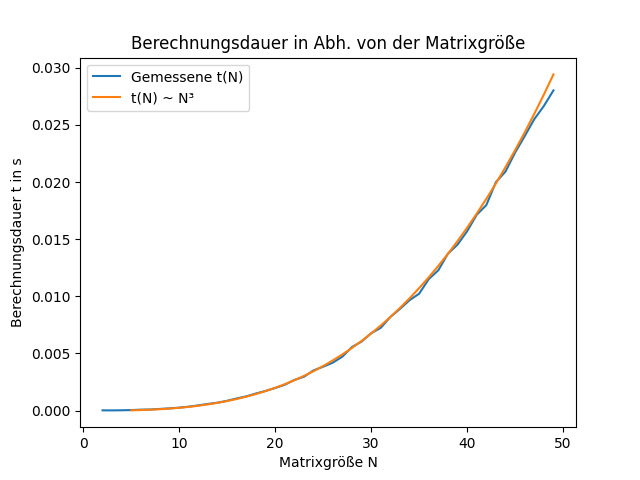
\includegraphics[width=0.5\textwidth]{fig1}
		\caption{Berechnungsdauer $t$ in Abhängigkeit von der Matrixgröße $N$}
	\end{wrapfigure}
	Meine Behauptung, dass die LU-Zerlegung $O(n^3)$ dauert, kann man sehr schön anhand der Abbildung 1 verifizieren. Dort ist die Berechnungsdauer $t$ von der LU-Zerlegung in Abhängigkeit von der Matrixgröße $N$ (bedeutet, dass immer $N\times N$ - Matrizen zerlegt werden) abgezeichnet. Es zeigt sich, dass die gemessenen Zeiten sehr gut proportional zu $N^3$ ist. Der orangene Graph ist um genau zu sein
	$$t(N) = 2.5 \cdot 10^{-7} \cdot N^3$$
	Das $O(n^3)$ Verhalten kommt daher, dass für jede Spalte im Mittel durch die Hälfte aller Zeilen und dann nochmal im Mittel die Hälfte aller Spalten iteriert werden muss.

\end{document}
